\documentclass[10pt,a4j,dvipdfmx]{jsarticle}
\usepackage[utf8]{inputenc}
\usepackage[dvipdfmx]{graphicx}
\usepackage[usenames,dvipdfmx]{color}
\usepackage{amsmath}
\usepackage{bm}
\usepackage[left=19.05mm, right=19.05mm, top=25.40mm, bottom=25.40mm]{geometry}
\usepackage{tikz}
\usepackage{circuitikz}
\usepackage{siunitx}
\usepackage{listings}
\usepackage{float}
\usepackage{hyperref}
\usepackage{enumitem}
\usepackage{textcomp}
\usepackage{gnuplot-lua-tikz}

\lstset{%
  language={C},
  basicstyle={\small},%
  identifierstyle={\small},%
  commentstyle={\small\itshape},%
  keywordstyle={\small\bfseries},%
  ndkeywordstyle={\small},%
  stringstyle={\small\ttfamily},
  frame={tb},
  breaklines=true,
  columns=[l]{fullflexible},%
  numbers=left,%
  xrightmargin=0zw,%
  xleftmargin=3zw,%
  numberstyle={\scriptsize},%
  stepnumber=1,
  numbersep=1zw,%
  lineskip=-0.5ex%
}

\usepackage{fouriernc}
\usepackage[scaled]{helvet}
\usepackage[T1]{fontenc}
\renewcommand{\ttdefault}{fvm}

\let\oldthefootnote\thefootnote
\def\thefootnote{{\color{Magenta}\oldthefootnote}}

\newcommand{\enhance}[1]{{\gtfamily\sffamily#1}}
\makeatletter
\def\@jikkenname{}
\def\@jikkennum{}
\def\@reportname{}
\def\@studentnumber{}
\def\@studentname{}
\def\@studentdepartment{}
\def\@friendnames{}
\def\@groupnumber{}
\newcommand{\jikkenset}[2]{\def\@jikkennum{#1}\def\@jikkenname{#2}}
\newcommand{\studentset}[3]{\def\@studentnumber{#1}\def\@studentname{#2}\def\@studentdepartment{#3}}
\newcommand{\reportnameset}[1]{\def\@reportname{#1}}
\newcommand{\friendname}[1]{\def\@friendnames{#1}}
\newcommand{\groupnumber}[1]{\def\@groupnumber{#1}}
\renewcommand{\maketitle}{
\noindent{\color{RoyalPurple}\hrule height 1pt \hfill}
\vspace{5pt}
\begin{center}
\enhance{{\Large{電気電子情報第一(前期)実験}}}\\[7pt]
\enhance{{\Huge\textbf{\@jikkennum{}. \@jikkenname}}}\\[5pt]
\enhance{{\LARGE{\@reportname}}}\\[15pt]
\@studentnumber\ \ \ \@studentname{}(\@studentdepartment{})\\[1pt]
共同実験者: \@friendnames(第\@groupnumber{}班)\\[1pt]
\today
\end{center}
\vspace{-10pt}
\noindent{\color{RoyalPurple}\hrule height 1pt \hfill}
}
\makeatother
\jikkenset{I1}{情報: 第1部}
\reportnameset{考察レポート}
\studentset{03-160441}{土屋潤一郎}{工学部 電子情報工学科}
\friendname{井上友貴、田中大幹、坂口達彦}
\groupnumber{28}

\makeatletter
\let\@oldsec\section
\let\@oldsubsec\subsection
\renewcommand{\section}[1]{\@oldsec{#1}\vspace{-5pt}{\color{TealBlue}\hrule height 0.6pt \hfill}\par}
\renewcommand{\thesection}{\arabic{section}.}
\renewcommand{\subsection}[1]{\vspace{-7pt}\@oldsubsec{#1}}
\makeatother

\begin{document}
\maketitle

\section{実験の概要}
\begin{description}
 \item[第1日]Linuxコマンド及びEmacsの使用法の復習、C言語プログラムのデバッグを通してのデバッガの使用法の復習
 \item[第2日]低水準入出力関数を用いたファイルの入出力、raw形式を主とした音声データの取り扱い
 \item[第3日]実習時間
 \item[第4日]ダウンサンプリングによるナイキスト周波数の実感、高速フーリエ変換を用いたデジタルフィルタの作成
\end{description}
\section{考察}
\subsection{低水準入出力関数}
第2日に、低水準入出力関数を用いてファイルの読み書きを行った。
低水準入出力関数では、OSのシステムコールを直接呼び出すことでファイルを取り扱う。
重要なのは、C言語に標準的に用意されている高水準入出力関数と異なり、メモリにバッファを用意しない。
このため、これらの命令が何度も繰り返されるような場面では、何度もディスク(の目的のファイル領域)へのアクセスが発生し低速になるが、一方で、複数のプロセスが一つのファイルを同時に扱うような場合、入出力が意図した時系列順に行われる。
従って、一連のメモリ領域に一度にデータを溜め込みたい場合や、逆に一連のメモリ領域から一度にデータを吐き出したい場合には、低水準入出力関数を用いて可能な限り意図した時系列で動作を行わせることができる。
また、低水準入出力関数では、そのサイズ指定をバイト単位で行うことから、よりバイナリを意識することが必要である。
これらのうち、入出力メモリバッファの有無を確認するために、簡単な比較実験を以下のように行った。

特定のファイルをオープンし、そのファイルに(配列に格納した)$10^6$byteの0を書き込む。
これを、
\begin{enumerate}
\item 低水準(write)・1byteずつ(つまり、writeを$10^6$回呼び出す)
\item 低水準(write)・一度に$10^6$byteまとめて
\item 高水準(fwrite)・1byteずつ
\item 高水準(fwrite)・一度に$10^6$byteまとめて
 \end{enumerate}
という条件で行い、C言語標準の<time.h>を用いて時間を計測する。
その結果が以下の通りである。
\begin{enumerate}
\item \SI{1127.59}{\milli\second}
\item \SI{9.45}{\milli\second}
\item \SI{31.29}{\milli\second}
\item \SI{9.46}{\milli\second}
\end{enumerate}
やはり低水準出力関数を複数回実行するとその分だけ時間がかかっていることがわかる。
高水準出力関数を用いてもこの傾向は見られるが、これは出力のメモリバッファがプログラム実行途中でいっぱいになってしまい、複数回書き込みをしているためだと考えられるが、その回数は低水準出力関数を用いた時よりも明らかに少ないことがわかる。

\subsection{ダウンサンプリングとナイキスト周波数}
第4日に、正弦波をサンプリングした値列から、n個に一個の割合で標本を抜き出してきて新たに標本値列を作成した。
これは、標本化周波数を$n^{-1}$倍するのに等しい。
この際、標本化周波数の1/2の値を持つナイキスト周波数以上の周波数は正しく復元できない。

そこで今回は、基本のAの2オクターブ上のA、すなわち\SI{1760}{\hertz}の正弦波の2種のダウンサンプリングを行った。
標本化周波数を$\frac{44100}{10} = 4410[\si{\hertz}]$にする、標本値列から10個に1個の割合で値を抜き出してくる方法と、標本化周波数を$\frac{44100}{15} = 2940[\si{\hertz}]$にする、標本値列から15個に1個の割合で値を抜き出してくる方法とである。
以下図1がその様子である。

\begin{figure}[H]
\centering
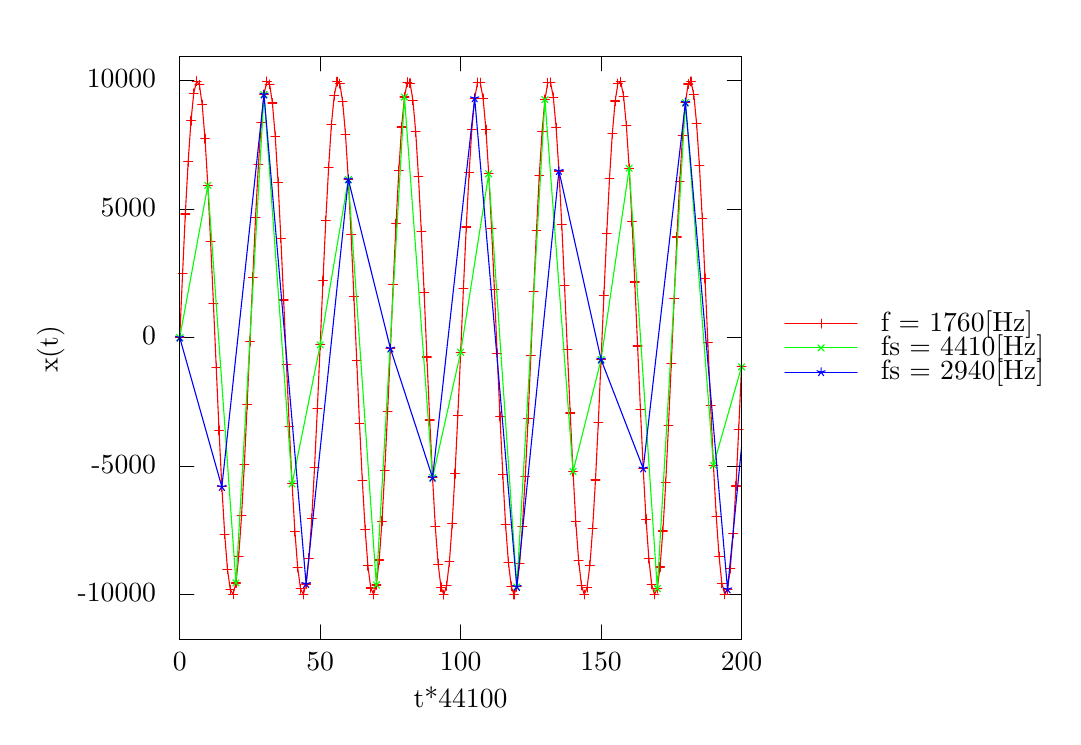
\begin{tikzpicture}[gnuplot]
%% generated with GNUPLOT 4.6p4 (Lua 5.1; terminal rev. 99, script rev. 100)
%% 2016年06月03日 18時23分37秒
\path (0.000,0.000) rectangle (12.500,8.750);
\gpcolor{color=gp lt color border}
\gpsetlinetype{gp lt border}
\gpsetlinewidth{1.00}
\draw[gp path] (1.872,1.550)--(2.052,1.550);
\draw[gp path] (9.007,1.550)--(8.827,1.550);
\node[gp node right] at (1.688,1.550) {-10000};
\draw[gp path] (1.872,3.182)--(2.052,3.182);
\draw[gp path] (9.007,3.182)--(8.827,3.182);
\node[gp node right] at (1.688,3.182) {-5000};
\draw[gp path] (1.872,4.814)--(2.052,4.814);
\draw[gp path] (9.007,4.814)--(8.827,4.814);
\node[gp node right] at (1.688,4.814) { 0};
\draw[gp path] (1.872,6.446)--(2.052,6.446);
\draw[gp path] (9.007,6.446)--(8.827,6.446);
\node[gp node right] at (1.688,6.446) { 5000};
\draw[gp path] (1.872,8.078)--(2.052,8.078);
\draw[gp path] (9.007,8.078)--(8.827,8.078);
\node[gp node right] at (1.688,8.078) { 10000};
\draw[gp path] (1.872,0.985)--(1.872,1.165);
\draw[gp path] (1.872,8.381)--(1.872,8.201);
\node[gp node center] at (1.872,0.677) { 0};
\draw[gp path] (3.656,0.985)--(3.656,1.165);
\draw[gp path] (3.656,8.381)--(3.656,8.201);
\node[gp node center] at (3.656,0.677) { 50};
\draw[gp path] (5.440,0.985)--(5.440,1.165);
\draw[gp path] (5.440,8.381)--(5.440,8.201);
\node[gp node center] at (5.440,0.677) { 100};
\draw[gp path] (7.223,0.985)--(7.223,1.165);
\draw[gp path] (7.223,8.381)--(7.223,8.201);
\node[gp node center] at (7.223,0.677) { 150};
\draw[gp path] (9.007,0.985)--(9.007,1.165);
\draw[gp path] (9.007,8.381)--(9.007,8.201);
\node[gp node center] at (9.007,0.677) { 200};
\draw[gp path] (1.872,8.381)--(1.872,0.985)--(9.007,0.985)--(9.007,8.381)--cycle;
\node[gp node center,rotate=-270] at (0.246,4.683) {x(t)};
\node[gp node center] at (5.439,0.215) {t*44100};
\node[gp node left] at (10.659,4.991) {f = 1760[Hz]};
\gpcolor{color=gp lt color 0}
\gpsetlinetype{gp lt plot 0}
\draw[gp path] (9.559,4.991)--(10.475,4.991);
\draw[gp path] (1.872,4.814)--(1.908,5.624)--(1.943,6.384)--(1.979,7.045)--(2.015,7.566)%
  --(2.050,7.916)--(2.086,8.071)--(2.122,8.023)--(2.157,7.774)--(2.193,7.340)--(2.229,6.748)%
  --(2.264,6.035)--(2.300,5.245)--(2.336,4.429)--(2.371,3.637)--(2.407,2.918)--(2.443,2.318)%
  --(2.478,1.874)--(2.514,1.614)--(2.550,1.555)--(2.586,1.698)--(2.621,2.037)--(2.657,2.550)%
  --(2.693,3.204)--(2.728,3.959)--(2.764,4.768)--(2.800,5.579)--(2.835,6.342)--(2.871,7.010)%
  --(2.907,7.541)--(2.942,7.901)--(2.978,8.068)--(3.014,8.031)--(3.049,7.793)--(3.085,7.369)%
  --(3.121,6.785)--(3.156,6.078)--(3.192,5.291)--(3.228,4.475)--(3.263,3.680)--(3.299,2.956)%
  --(3.335,2.348)--(3.370,1.895)--(3.406,1.624)--(3.442,1.552)--(3.477,1.685)--(3.513,2.013)%
  --(3.549,2.517)--(3.584,3.164)--(3.620,3.915)--(3.656,4.721)--(3.691,5.534)--(3.727,6.301)%
  --(3.763,6.976)--(3.798,7.515)--(3.834,7.885)--(3.870,8.064)--(3.905,8.039)--(3.941,7.812)%
  --(3.977,7.398)--(4.013,6.822)--(4.048,6.120)--(4.084,5.337)--(4.120,4.522)--(4.155,3.724)%
  --(4.191,2.995)--(4.227,2.379)--(4.262,1.916)--(4.298,1.634)--(4.334,1.551)--(4.369,1.672)%
  --(4.405,1.990)--(4.441,2.484)--(4.476,3.124)--(4.512,3.870)--(4.548,4.675)--(4.583,5.488)%
  --(4.619,6.260)--(4.655,6.941)--(4.690,7.489)--(4.726,7.869)--(4.762,8.059)--(4.797,8.046)%
  --(4.833,7.830)--(4.869,7.426)--(4.904,6.859)--(4.940,6.163)--(4.976,5.383)--(5.011,4.568)%
  --(5.047,3.768)--(5.083,3.034)--(5.118,2.410)--(5.154,1.937)--(5.190,1.645)--(5.225,1.550)%
  --(5.261,1.660)--(5.297,1.966)--(5.332,2.452)--(5.368,3.084)--(5.404,3.825)--(5.440,4.628)%
  --(5.475,5.443)--(5.511,6.218)--(5.547,6.905)--(5.582,7.462)--(5.618,7.853)--(5.654,8.054)%
  --(5.689,8.052)--(5.725,7.848)--(5.761,7.454)--(5.796,6.894)--(5.832,6.205)--(5.868,5.429)%
  --(5.903,4.614)--(5.939,3.812)--(5.975,3.073)--(6.010,2.442)--(6.046,1.960)--(6.082,1.656)%
  --(6.117,1.550)--(6.153,1.648)--(6.189,1.944)--(6.224,2.420)--(6.260,3.045)--(6.296,3.781)%
  --(6.331,4.582)--(6.367,5.397)--(6.403,6.176)--(6.438,6.869)--(6.474,7.434)--(6.510,7.836)%
  --(6.545,8.048)--(6.581,8.057)--(6.617,7.865)--(6.652,7.481)--(6.688,6.930)--(6.724,6.247)%
  --(6.759,5.475)--(6.795,4.661)--(6.831,3.856)--(6.867,3.112)--(6.902,2.474)--(6.938,1.983)%
  --(6.974,1.668)--(7.009,1.551)--(7.045,1.637)--(7.081,1.922)--(7.116,2.389)--(7.152,3.006)%
  --(7.188,3.737)--(7.223,4.535)--(7.259,5.351)--(7.295,6.133)--(7.330,6.833)--(7.366,7.406)%
  --(7.402,7.818)--(7.437,8.041)--(7.473,8.062)--(7.509,7.881)--(7.544,7.507)--(7.580,6.965)%
  --(7.616,6.289)--(7.651,5.520)--(7.687,4.707)--(7.723,3.901)--(7.758,3.152)--(7.794,2.507)%
  --(7.830,2.006)--(7.865,1.681)--(7.901,1.552)--(7.937,1.627)--(7.972,1.901)--(8.008,2.358)%
  --(8.044,2.968)--(8.079,3.693)--(8.115,4.489)--(8.151,5.305)--(8.186,6.091)--(8.222,6.796)%
  --(8.258,7.378)--(8.294,7.799)--(8.329,8.034)--(8.365,8.067)--(8.401,7.896)--(8.436,7.533)%
  --(8.472,7.000)--(8.508,6.330)--(8.543,5.566)--(8.579,4.754)--(8.615,3.946)--(8.650,3.192)%
  --(8.686,2.540)--(8.722,2.030)--(8.757,1.694)--(8.793,1.554)--(8.829,1.617)--(8.864,1.880)%
  --(8.900,2.327)--(8.936,2.929)--(8.971,3.650)--(9.007,4.443);
\gpsetpointsize{4.00}
\gppoint{gp mark 1}{(1.872,4.814)}
\gppoint{gp mark 1}{(1.908,5.624)}
\gppoint{gp mark 1}{(1.943,6.384)}
\gppoint{gp mark 1}{(1.979,7.045)}
\gppoint{gp mark 1}{(2.015,7.566)}
\gppoint{gp mark 1}{(2.050,7.916)}
\gppoint{gp mark 1}{(2.086,8.071)}
\gppoint{gp mark 1}{(2.122,8.023)}
\gppoint{gp mark 1}{(2.157,7.774)}
\gppoint{gp mark 1}{(2.193,7.340)}
\gppoint{gp mark 1}{(2.229,6.748)}
\gppoint{gp mark 1}{(2.264,6.035)}
\gppoint{gp mark 1}{(2.300,5.245)}
\gppoint{gp mark 1}{(2.336,4.429)}
\gppoint{gp mark 1}{(2.371,3.637)}
\gppoint{gp mark 1}{(2.407,2.918)}
\gppoint{gp mark 1}{(2.443,2.318)}
\gppoint{gp mark 1}{(2.478,1.874)}
\gppoint{gp mark 1}{(2.514,1.614)}
\gppoint{gp mark 1}{(2.550,1.555)}
\gppoint{gp mark 1}{(2.586,1.698)}
\gppoint{gp mark 1}{(2.621,2.037)}
\gppoint{gp mark 1}{(2.657,2.550)}
\gppoint{gp mark 1}{(2.693,3.204)}
\gppoint{gp mark 1}{(2.728,3.959)}
\gppoint{gp mark 1}{(2.764,4.768)}
\gppoint{gp mark 1}{(2.800,5.579)}
\gppoint{gp mark 1}{(2.835,6.342)}
\gppoint{gp mark 1}{(2.871,7.010)}
\gppoint{gp mark 1}{(2.907,7.541)}
\gppoint{gp mark 1}{(2.942,7.901)}
\gppoint{gp mark 1}{(2.978,8.068)}
\gppoint{gp mark 1}{(3.014,8.031)}
\gppoint{gp mark 1}{(3.049,7.793)}
\gppoint{gp mark 1}{(3.085,7.369)}
\gppoint{gp mark 1}{(3.121,6.785)}
\gppoint{gp mark 1}{(3.156,6.078)}
\gppoint{gp mark 1}{(3.192,5.291)}
\gppoint{gp mark 1}{(3.228,4.475)}
\gppoint{gp mark 1}{(3.263,3.680)}
\gppoint{gp mark 1}{(3.299,2.956)}
\gppoint{gp mark 1}{(3.335,2.348)}
\gppoint{gp mark 1}{(3.370,1.895)}
\gppoint{gp mark 1}{(3.406,1.624)}
\gppoint{gp mark 1}{(3.442,1.552)}
\gppoint{gp mark 1}{(3.477,1.685)}
\gppoint{gp mark 1}{(3.513,2.013)}
\gppoint{gp mark 1}{(3.549,2.517)}
\gppoint{gp mark 1}{(3.584,3.164)}
\gppoint{gp mark 1}{(3.620,3.915)}
\gppoint{gp mark 1}{(3.656,4.721)}
\gppoint{gp mark 1}{(3.691,5.534)}
\gppoint{gp mark 1}{(3.727,6.301)}
\gppoint{gp mark 1}{(3.763,6.976)}
\gppoint{gp mark 1}{(3.798,7.515)}
\gppoint{gp mark 1}{(3.834,7.885)}
\gppoint{gp mark 1}{(3.870,8.064)}
\gppoint{gp mark 1}{(3.905,8.039)}
\gppoint{gp mark 1}{(3.941,7.812)}
\gppoint{gp mark 1}{(3.977,7.398)}
\gppoint{gp mark 1}{(4.013,6.822)}
\gppoint{gp mark 1}{(4.048,6.120)}
\gppoint{gp mark 1}{(4.084,5.337)}
\gppoint{gp mark 1}{(4.120,4.522)}
\gppoint{gp mark 1}{(4.155,3.724)}
\gppoint{gp mark 1}{(4.191,2.995)}
\gppoint{gp mark 1}{(4.227,2.379)}
\gppoint{gp mark 1}{(4.262,1.916)}
\gppoint{gp mark 1}{(4.298,1.634)}
\gppoint{gp mark 1}{(4.334,1.551)}
\gppoint{gp mark 1}{(4.369,1.672)}
\gppoint{gp mark 1}{(4.405,1.990)}
\gppoint{gp mark 1}{(4.441,2.484)}
\gppoint{gp mark 1}{(4.476,3.124)}
\gppoint{gp mark 1}{(4.512,3.870)}
\gppoint{gp mark 1}{(4.548,4.675)}
\gppoint{gp mark 1}{(4.583,5.488)}
\gppoint{gp mark 1}{(4.619,6.260)}
\gppoint{gp mark 1}{(4.655,6.941)}
\gppoint{gp mark 1}{(4.690,7.489)}
\gppoint{gp mark 1}{(4.726,7.869)}
\gppoint{gp mark 1}{(4.762,8.059)}
\gppoint{gp mark 1}{(4.797,8.046)}
\gppoint{gp mark 1}{(4.833,7.830)}
\gppoint{gp mark 1}{(4.869,7.426)}
\gppoint{gp mark 1}{(4.904,6.859)}
\gppoint{gp mark 1}{(4.940,6.163)}
\gppoint{gp mark 1}{(4.976,5.383)}
\gppoint{gp mark 1}{(5.011,4.568)}
\gppoint{gp mark 1}{(5.047,3.768)}
\gppoint{gp mark 1}{(5.083,3.034)}
\gppoint{gp mark 1}{(5.118,2.410)}
\gppoint{gp mark 1}{(5.154,1.937)}
\gppoint{gp mark 1}{(5.190,1.645)}
\gppoint{gp mark 1}{(5.225,1.550)}
\gppoint{gp mark 1}{(5.261,1.660)}
\gppoint{gp mark 1}{(5.297,1.966)}
\gppoint{gp mark 1}{(5.332,2.452)}
\gppoint{gp mark 1}{(5.368,3.084)}
\gppoint{gp mark 1}{(5.404,3.825)}
\gppoint{gp mark 1}{(5.440,4.628)}
\gppoint{gp mark 1}{(5.475,5.443)}
\gppoint{gp mark 1}{(5.511,6.218)}
\gppoint{gp mark 1}{(5.547,6.905)}
\gppoint{gp mark 1}{(5.582,7.462)}
\gppoint{gp mark 1}{(5.618,7.853)}
\gppoint{gp mark 1}{(5.654,8.054)}
\gppoint{gp mark 1}{(5.689,8.052)}
\gppoint{gp mark 1}{(5.725,7.848)}
\gppoint{gp mark 1}{(5.761,7.454)}
\gppoint{gp mark 1}{(5.796,6.894)}
\gppoint{gp mark 1}{(5.832,6.205)}
\gppoint{gp mark 1}{(5.868,5.429)}
\gppoint{gp mark 1}{(5.903,4.614)}
\gppoint{gp mark 1}{(5.939,3.812)}
\gppoint{gp mark 1}{(5.975,3.073)}
\gppoint{gp mark 1}{(6.010,2.442)}
\gppoint{gp mark 1}{(6.046,1.960)}
\gppoint{gp mark 1}{(6.082,1.656)}
\gppoint{gp mark 1}{(6.117,1.550)}
\gppoint{gp mark 1}{(6.153,1.648)}
\gppoint{gp mark 1}{(6.189,1.944)}
\gppoint{gp mark 1}{(6.224,2.420)}
\gppoint{gp mark 1}{(6.260,3.045)}
\gppoint{gp mark 1}{(6.296,3.781)}
\gppoint{gp mark 1}{(6.331,4.582)}
\gppoint{gp mark 1}{(6.367,5.397)}
\gppoint{gp mark 1}{(6.403,6.176)}
\gppoint{gp mark 1}{(6.438,6.869)}
\gppoint{gp mark 1}{(6.474,7.434)}
\gppoint{gp mark 1}{(6.510,7.836)}
\gppoint{gp mark 1}{(6.545,8.048)}
\gppoint{gp mark 1}{(6.581,8.057)}
\gppoint{gp mark 1}{(6.617,7.865)}
\gppoint{gp mark 1}{(6.652,7.481)}
\gppoint{gp mark 1}{(6.688,6.930)}
\gppoint{gp mark 1}{(6.724,6.247)}
\gppoint{gp mark 1}{(6.759,5.475)}
\gppoint{gp mark 1}{(6.795,4.661)}
\gppoint{gp mark 1}{(6.831,3.856)}
\gppoint{gp mark 1}{(6.867,3.112)}
\gppoint{gp mark 1}{(6.902,2.474)}
\gppoint{gp mark 1}{(6.938,1.983)}
\gppoint{gp mark 1}{(6.974,1.668)}
\gppoint{gp mark 1}{(7.009,1.551)}
\gppoint{gp mark 1}{(7.045,1.637)}
\gppoint{gp mark 1}{(7.081,1.922)}
\gppoint{gp mark 1}{(7.116,2.389)}
\gppoint{gp mark 1}{(7.152,3.006)}
\gppoint{gp mark 1}{(7.188,3.737)}
\gppoint{gp mark 1}{(7.223,4.535)}
\gppoint{gp mark 1}{(7.259,5.351)}
\gppoint{gp mark 1}{(7.295,6.133)}
\gppoint{gp mark 1}{(7.330,6.833)}
\gppoint{gp mark 1}{(7.366,7.406)}
\gppoint{gp mark 1}{(7.402,7.818)}
\gppoint{gp mark 1}{(7.437,8.041)}
\gppoint{gp mark 1}{(7.473,8.062)}
\gppoint{gp mark 1}{(7.509,7.881)}
\gppoint{gp mark 1}{(7.544,7.507)}
\gppoint{gp mark 1}{(7.580,6.965)}
\gppoint{gp mark 1}{(7.616,6.289)}
\gppoint{gp mark 1}{(7.651,5.520)}
\gppoint{gp mark 1}{(7.687,4.707)}
\gppoint{gp mark 1}{(7.723,3.901)}
\gppoint{gp mark 1}{(7.758,3.152)}
\gppoint{gp mark 1}{(7.794,2.507)}
\gppoint{gp mark 1}{(7.830,2.006)}
\gppoint{gp mark 1}{(7.865,1.681)}
\gppoint{gp mark 1}{(7.901,1.552)}
\gppoint{gp mark 1}{(7.937,1.627)}
\gppoint{gp mark 1}{(7.972,1.901)}
\gppoint{gp mark 1}{(8.008,2.358)}
\gppoint{gp mark 1}{(8.044,2.968)}
\gppoint{gp mark 1}{(8.079,3.693)}
\gppoint{gp mark 1}{(8.115,4.489)}
\gppoint{gp mark 1}{(8.151,5.305)}
\gppoint{gp mark 1}{(8.186,6.091)}
\gppoint{gp mark 1}{(8.222,6.796)}
\gppoint{gp mark 1}{(8.258,7.378)}
\gppoint{gp mark 1}{(8.294,7.799)}
\gppoint{gp mark 1}{(8.329,8.034)}
\gppoint{gp mark 1}{(8.365,8.067)}
\gppoint{gp mark 1}{(8.401,7.896)}
\gppoint{gp mark 1}{(8.436,7.533)}
\gppoint{gp mark 1}{(8.472,7.000)}
\gppoint{gp mark 1}{(8.508,6.330)}
\gppoint{gp mark 1}{(8.543,5.566)}
\gppoint{gp mark 1}{(8.579,4.754)}
\gppoint{gp mark 1}{(8.615,3.946)}
\gppoint{gp mark 1}{(8.650,3.192)}
\gppoint{gp mark 1}{(8.686,2.540)}
\gppoint{gp mark 1}{(8.722,2.030)}
\gppoint{gp mark 1}{(8.757,1.694)}
\gppoint{gp mark 1}{(8.793,1.554)}
\gppoint{gp mark 1}{(8.829,1.617)}
\gppoint{gp mark 1}{(8.864,1.880)}
\gppoint{gp mark 1}{(8.900,2.327)}
\gppoint{gp mark 1}{(8.936,2.929)}
\gppoint{gp mark 1}{(8.971,3.650)}
\gppoint{gp mark 1}{(9.007,4.443)}
\gppoint{gp mark 1}{(10.017,4.991)}
\gpcolor{color=gp lt color border}
\node[gp node left] at (10.659,4.683) {fs = 4410[Hz]};
\gpcolor{color=gp lt color 1}
\gpsetlinetype{gp lt plot 1}
\draw[gp path] (9.559,4.683)--(10.475,4.683);
\draw[gp path] (1.872,4.814)--(2.229,6.748)--(2.586,1.698)--(2.942,7.901)--(3.299,2.956)%
  --(3.656,4.721)--(4.013,6.822)--(4.369,1.672)--(4.726,7.869)--(5.083,3.034)--(5.440,4.628)%
  --(5.796,6.894)--(6.153,1.648)--(6.510,7.836)--(6.867,3.112)--(7.223,4.535)--(7.580,6.965)%
  --(7.937,1.627)--(8.294,7.799)--(8.650,3.192)--(9.007,4.443);
\gppoint{gp mark 2}{(1.872,4.814)}
\gppoint{gp mark 2}{(2.229,6.748)}
\gppoint{gp mark 2}{(2.586,1.698)}
\gppoint{gp mark 2}{(2.942,7.901)}
\gppoint{gp mark 2}{(3.299,2.956)}
\gppoint{gp mark 2}{(3.656,4.721)}
\gppoint{gp mark 2}{(4.013,6.822)}
\gppoint{gp mark 2}{(4.369,1.672)}
\gppoint{gp mark 2}{(4.726,7.869)}
\gppoint{gp mark 2}{(5.083,3.034)}
\gppoint{gp mark 2}{(5.440,4.628)}
\gppoint{gp mark 2}{(5.796,6.894)}
\gppoint{gp mark 2}{(6.153,1.648)}
\gppoint{gp mark 2}{(6.510,7.836)}
\gppoint{gp mark 2}{(6.867,3.112)}
\gppoint{gp mark 2}{(7.223,4.535)}
\gppoint{gp mark 2}{(7.580,6.965)}
\gppoint{gp mark 2}{(7.937,1.627)}
\gppoint{gp mark 2}{(8.294,7.799)}
\gppoint{gp mark 2}{(8.650,3.192)}
\gppoint{gp mark 2}{(9.007,4.443)}
\gppoint{gp mark 2}{(10.017,4.683)}
\gpcolor{color=gp lt color border}
\node[gp node left] at (10.659,4.375) {fs = 2940[Hz]};
\gpcolor{color=gp lt color 2}
\gpsetlinetype{gp lt plot 2}
\draw[gp path] (9.559,4.375)--(10.475,4.375);
\draw[gp path] (1.872,4.814)--(2.407,2.918)--(2.942,7.901)--(3.477,1.685)--(4.013,6.822)%
  --(4.548,4.675)--(5.083,3.034)--(5.618,7.853)--(6.153,1.648)--(6.688,6.930)--(7.223,4.535)%
  --(7.758,3.152)--(8.294,7.799)--(8.829,1.617)--(9.007,3.423);
\gppoint{gp mark 3}{(1.872,4.814)}
\gppoint{gp mark 3}{(2.407,2.918)}
\gppoint{gp mark 3}{(2.942,7.901)}
\gppoint{gp mark 3}{(3.477,1.685)}
\gppoint{gp mark 3}{(4.013,6.822)}
\gppoint{gp mark 3}{(4.548,4.675)}
\gppoint{gp mark 3}{(5.083,3.034)}
\gppoint{gp mark 3}{(5.618,7.853)}
\gppoint{gp mark 3}{(6.153,1.648)}
\gppoint{gp mark 3}{(6.688,6.930)}
\gppoint{gp mark 3}{(7.223,4.535)}
\gppoint{gp mark 3}{(7.758,3.152)}
\gppoint{gp mark 3}{(8.294,7.799)}
\gppoint{gp mark 3}{(8.829,1.617)}
\gppoint{gp mark 3}{(10.017,4.375)}
\gpcolor{color=gp lt color border}
\gpsetlinetype{gp lt border}
\draw[gp path] (1.872,8.381)--(1.872,0.985)--(9.007,0.985)--(9.007,8.381)--cycle;
%% coordinates of the plot area
\gpdefrectangularnode{gp plot 1}{\pgfpoint{1.872cm}{0.985cm}}{\pgfpoint{9.007cm}{8.381cm}}
\end{tikzpicture}
%% gnuplot variables

\caption{ダウンサンプリングの結果}
\label{fig:label}
\end{figure}

緑の破線が示す、標本化周波数\SI{4410}{\hertz}のグラフは、もとの赤い線が示す正弦波の山と谷を捉えきれている、と言える。
一方、青の破線が示す、標本化周波数\SI{2940}{\hertz}のグラフは、もとの赤い線が示す正弦波の山と谷を明らかに捉えきれていない。
\SI{1760}{\hertz}をナイキスト周波数として復元可能域に含めるためには、標本化周波数は\SI{3520}{\hertz}でなければならないことを、(簡易的にであるが)確認することができた。
また、人間の可聴域の上限がおおよそ\SI{20,000}{\hertz}なので、CDなどの標本化周波数は\SI{44,100}{\hertz}が用いられるが、今後音声電話を作成していく際には、これにとらわれず、ある程度(周波数フィルタによって)高音域を諦めることで標本値列のデータ量を減らせることがわかる。

\section{参考資料}
\begin{enumerate}
\item 東京大学工学部電子情報工学科・電気電子工学科(2016)『電気電子情報第一(前期)実験テキスト』
\end{enumerate}

\end{document}
